% Template for ICASSP-2021 paper; to be used with:
%          spconf.sty  - ICASSP/ICIP LaTeX style file, and
%          IEEEbib.bst - IEEE bibliography style file.
% --------------------------------------------------------------------------
\documentclass{article}
\usepackage{spconf,amsmath,graphicx,makecell,url}
\usepackage{color}
\usepackage{ulem}
\usepackage{soul}
\usepackage{booktabs}
\usepackage{multirow}

% Title.
% ------
\title{Prompt-Distiller: Few-shot Knowledge Distillation for Prompt-based Language Learners with Dual Contrastive Learning}
%
% Single address.
% ---------------
\name{Boyu Hou\textsuperscript{1}\thanks{Boyu Hou and Chengyu Wang contributed equally to this work.}, Chengyu Wang\textsuperscript{2}, Xiaoqing Chen\textsuperscript{1}, Minghui Qiu\textsuperscript{2,\textdagger}\thanks{\textdagger~Corresponding authors: Liang Feng (\url{liangf@cqu.edu.cn}) and Minghui Qiu (\url{minghui.qmh@alibaba-inc.com}).}, Liang Feng\textsuperscript{1,\textdagger}, Jun Huang\textsuperscript{2}}
\address{\textsuperscript{1} College of Computer Science, Chongqing University, Chongqing, China\\
\textsuperscript{2} Alibaba Group, Hangzhou, China}


\begin{document}
\maketitle

\begin{abstract}
	Prompt-based learning has improved the few-shot learning performance of large-scale Pre-trained Language Models (PLMs). Yet, it is challenging to deploy large-scale PLMs in resource-constrained environments for online applications. Knowledge Distillation (KD) is a promising approach for PLM compression. However, distilling prompt-tuned PLMs in the few-shot learning setting is a non-trivial problem due to the lack of task-specific training data and KD techniques for the new prompting paradigm.
	We propose Prompt-Distiller, the first few-shot KD algorithm for prompt-tuned PLMs, which forces the student model to learn from both its pre-trained and prompt-tuned teacher models to alleviate the model overfitting problem.
	We further design a contrastive learning technique to learn higher-order dependencies from intermediate-layer representations of teacher models, considering different knowledge capacities of teacher and student models.
	Extensive experiments over various datasets show that Prompt-Distiller consistently outperforms baselines by a large margin.
	%\footnote{All the datasets are publicly available. Source codes will be released upon acceptance.}
\end{abstract}
%
\begin{keywords}
	knowledge distillation, few-shot learning, prompt-based learning, pre-trained language model
\end{keywords}
%

\begin{figure*}[t]
	\centering
	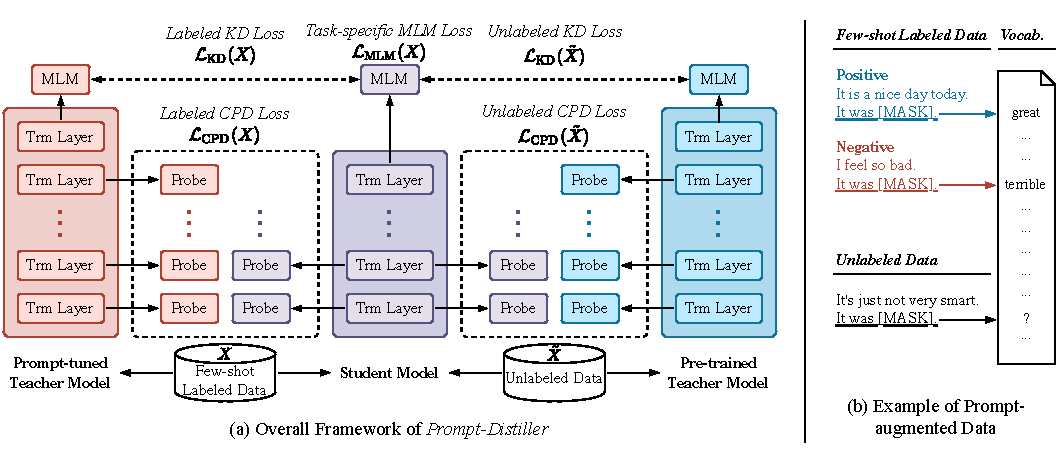
\includegraphics[width=\linewidth]{framework.pdf}
	\caption{An illustration of the Prompt-Distiller framework with examples of prompt-augmented data.}
	\label{fig:overview}
\end{figure*}


\section{Introduction}

Large-scale Pre-trained Language Models (PLMs) have significantly improved the performance of various downstream NLP tasks with the two-stage ``pre-training and fine-tuning'' paradigm~\cite{DBLP:journals/corr/abs-2003-08271,DBLP:journals/corr/abs-2106-07139}. Yet, a sufficiently large task-specific training set is required for model fine-tuning, which limits the applicability of PLMs.

Recently, prompt-based learning has been proposed to reformulate different NLP tasks uniformly as cloze questions and to provide additional task guidance by task-specific prompts~\cite{DBLP:journals/corr/abs-2107-13586}.
Notable works include PET~\cite{DBLP:conf/eacl/SchickS21}, LM-BFF~\cite{DBLP:conf/acl/GaoFC20},
AutoPrompt~\cite{DBLP:conf/emnlp/ShinRLWS20}, WARP~\cite{DBLP:conf/acl/HambardzumyanKM20},
P-tuning~\cite{DBLP:journals/corr/abs-2110-07602} and many others.
As prompting requires rich pre-training knowledge ``stored'' in PLMs by the Masked Language Modeling (MLM) task, larger PLMs typically have better few-shot performance.
%when prompt-based learning is applied.
Especially, ultra-large PLMs such as GPT-3~\cite{DBLP:journals/corr/abs-2109-07684}, Yuan 1.0~\cite{DBLP:journals/corr/abs-2110-04725} and FLAN~\cite{DBLP:journals/corr/abs-2109-01652} even have good zero-shot performance on previously unseen NLP tasks.


%, such as PET~\citep{schick-schutze-2021-exploiting}, reformulate the task as a cloze question and fine-tune with conventional gradient descent methods, which bring the downstream task and pre-training task closer together. Larger PLMs tend to have broader language knowledge, which could have a positive impact on Prompt-based Learning. There are several works that support this view~\citep{liu-2021-gpt,gao-2020-making}.

%each new task has a large labeled data requirement, which limits the applicability of PLMs. In order to make PLMs applications more efficient and economical,


%redirected research in the field of Natural Language Processing (NLP) and have greatly expanded the way natural language tasks can be applied. By designing unsupervised tasks such as Masked Language Model (MLM), large-scale PLMs as are able to model language over massive corpora \citep{devlin-2018-bert,liu-2019-roberta}. To apply PLMs to a downstream task, a typical approach is to use a task-specific header and fine-tune the entire model on a set of labeled data. From a practical point of view, each new task has a large labeled data requirement, which limits the applicability of PLMs. In order to make PLMs applications more efficient and economical, we seek to obtain comparable performance on a smaller labeled training set. The prompt-based learning methods, such as PET~\citep{schick-schutze-2021-exploiting}, reformulate the task as a cloze question and fine-tune with conventional gradient descent methods, which bring the downstream task and pre-training task closer together. Larger PLMs tend to have broader language knowledge, which could have a positive impact on Prompt-based Learning. There are several works that support this view~\citep{liu-2021-gpt,gao-2020-making}.

%However, larger PLMs lead to better performance while generating hundreds of millions of total parameters, and the size of the models is further increasing as various performance improvement schemes are proposed.

Unfortunately, the good performance of large models also means that it is challenging to deploy them online in resource-constrained environments, which introduce inference delays and large computation costs. A promising approach to address this issue is Knowledge Distillation (KD)~\cite{DBLP:journals/ijcv/GouYMT21}, which compresses a large model (i.e., the teacher model) into a small model (i.e., the student model), preserving the model performance while reducing the number of parameters.
However, distilling such models in few-shot learning settings is non-trivial for two reasons. i) Existing KD algorithms for BERT-like models such as vanilla KD~\cite{DBLP:journals/corr/abs-1903-12136}, Patient KD (PKD)~\cite{DBLP:conf/emnlp/SunCGL19} and TinyBERT~\cite{DBLP:conf/emnlp/JiaoYSJCL0L20} mostly focus on distilling the ``dark knolwedge'' (classification logits) and/or ``hints'' (intermediate representations) from the teacher model, which are not specifically designed for prompt-based PLMs. ii) In few-shot learning, the extreme lack of training data and the large parameter size of PLMs easily lead to severe overfitting of the student model.
Hence, a natural question arises:~\emph{how can we distill a prompt-based fine-tuned PLM to smaller models with few labeled training instances available?}

%This state of affairs has guided the research interest towards model compression methods. Knowledge distillation (KD) is a typical model compression method that compresses a large model (teacher model) into a small model (student model), preserving performance on downstream tasks while reducing the number of parameters and the number of operations. Recently, KD has been increasingly used in the NLP domain to address the deployment challenges posed by PLMs.

%The classical KD is based on dark knowledge to guide the training of student models, adding the difference in head logits between student and teacher networks as an auxiliary training target. On the other hand, using dark knowledge alone does not maintain the performance of compressed PLMs well, so some works have added intermediate layer representations (a.k.a. hints) as additional sources of knowledge. However, dark knowledge and hints cannot be directly applied to MLM-based prompt tuning for few-shot KD. Moreover, prompt tuning requires a sufficiently large teacher model, which can cause capacity gap problems and result in student networks not learning effective knowledge. Meanwhile, we found in our experiments that performance degradation often occurs in classical KD with few-shot scenarios. This may caused by a data starvation, where the student model receives supervised signals from a too single source and over-fitting occurs.

In this paper, we propose Prompt-Distiller, the first few-shot KD algorithm for prompt-based language learners. As the high performance of few-shot learners mostly result from the exploitation of pre-trained knowledge to downstream tasks, we force the MLM head of the student model to learn from both its pre-trained and prompt-tuned teacher models for the acquisition of task-specific and universal knowledge.
Specifically, the KD process of universal, pre-trained knowledge does not require any manually labeled data, which is suitable for few-shot learning.
We further design the probe-based contrastive learning technique to indirectly learn higher-order dependencies from intermediate-layer representations, where teacher and student models have significantly different capacities.
%We designed a dual learning of MLM head from both teacher PLM and teacher model to alleviate the over-fitting problem. MLM-based prompt tuning relies more on the knowledge in PLM rather than the few-shot labeled training dataset, we therefore used several times more homogeneous unlabeled corpus than labeled data to support the learning from teacher PLM. Next, we seek to use knowledge from the intermediate layer representations as much as possible by adding comparison targets to tap the higher-order dependencies between the BERT teachers and students.
We conduct extensive experiments over eight public datasets, associated with a variety of NLP tasks.
%such as sentiment analysis, natural language inference, question answering, etc.
Experiments show that Prompt-Distiller consistently outperforms baselines by a large margin.




\section{Prompt-Distiller: Proposed Approach}

We start with a brief overview of~{Prompt-Distiller}. After that, we elaborate the technical details.


\subsection{Overview}

For illustration, Prompt-Distiller and data samples are presented in Figure~\ref{fig:overview}.
Formally, given an $N$-way-$K$-shot training set $X=\{(x_i,y_i)\}$, together with a prompt-tuned PLM parameterized by ${\Theta}_{T}$, the goal of our work is to obtain a much smaller PLM parameterized by ${\Theta}_{S}$ such that the performance of ${\Theta}_{S}$ can be as close to ${\Theta}_{T}$ as possible.
Here, $y_i$ is the classification label of the input text $x_i$, where $\mathcal{Y}$ is the label set with $\vert\mathcal{Y}\vert=N$ and $y_i\in\mathcal{Y}$.
During parameter tuning, following~\cite{DBLP:conf/acl/GaoFC20}, we also have a few-shot development set that has the same size with $X$.
As the size of $X$ is extremely small (i.e.,~$N\times K$),
we also assume that there is a larger, unlabeled dataset $\tilde{X}=\{x_i\}$ with $\vert\tilde{X}\vert=n\cdot\vert X\vert$, serving as the auxiliary dataset for KD.
Without loss of generality, we use PET~\cite{DBLP:conf/eacl/SchickS21} to prompt-tune the teacher model on the training set $X$.
Hence, the entire workflow of obtaining teacher and student models only requires $N\times K$ labeled training samples.

%Hence, our work can learn a smaller model from a larger few-shot learner, where the entire workflow of obtaining the teacher and student models only requires $N\times K$ labeled samples.
%This is particularly useful in low-resourced scenarios.
%In the following, we describe the techniques of~\emph{Prompt-Distiller} in detail.

\begin{table*}
	\centering
	\begin{small}
		\begin{tabular}{c|l|cccccccc|c}
			\hline
			\textbf{Paradigm}   & \textbf{Method}                                     & \textbf{MNLI} & \textbf{MNLI-mm} & \textbf{MPQA} & \textbf{MR} & \textbf{RTE} & \textbf{SNLI} & \textbf{SST-2} & \textbf{TREC} & \textbf{Avg.} \\
			\hline
			\hline
			\multirow{5}{*}{FT} & \it Teacher FT (Upper Bound)                        & \it 44.3      & \it 46.3         & \it 66.3      & \it 75.0    & \it 50.5     & \it 48.5      & \it 79.7       & \it 85.3      & \it 61.9      \\
			                    & Student FT (Lower Bound)                            & 34.8          & 35.1             & 63.9          & 53.8        & 51.3         & 41.4          & 63.5           & 69.0          & 51.6          \\
			\cline{2-11}        & Vanilla KD~\cite{DBLP:journals/corr/abs-1903-12136} & 34.9          & 35.6             & 64.5          & 52.5        & 50.2         & 40.6          & 63.5           & 68.5          & 51.3          \\
			                    & BERT-PKD~\cite{DBLP:conf/emnlp/SunCGL19}            & 35.4          & 36.1             & 56.2          & 46.8        & 53.1         & 43.7          & 62.5           & 59.3          & 49.1          \\
			                    & TinyBERT~\cite{DBLP:conf/emnlp/JiaoYSJCL0L20}       & 35.6          & 36.4             & 64.7          & 48.8        & 53.3         & 42.8          & 63.5           & 63.2          & 51.0          \\
			\hline
			\multirow{4}{*}{PT} & \it Teacher PT (Upper Bound)                        & \it 67.0      & \it 69.0         & \it 84.5      & \it 87.0    & \it 71.3     & \it 77.3      & \it 93.1       & \it 85.8      & \it 79.3      \\
			                    & Student PT (Lower Bound)                            & 35.4          & 36.2             & 64.0          & 55.8        & 51.8         & 38.9          & 62.5           & 70.5          & 51.8          \\
			\cline{2-11}        & Prompt-KD                                           & 35.5          & 36.0             & 63.5          & 53.8        & 53.7         & 39.3          & 61.9           & 69.9          & 51.6          \\
			\cline{2-11}        & {\textbf{Prompt-Distiller (Ours)}}                  & \bf 43.3      & \bf 45.0         & \bf 75.5      & \bf 71.9    & \bf 55.6     & \bf 48.0      & \bf 78.4       & \bf 71.3      & \bf 61.1      \\
			\hline
		\end{tabular}
	\end{small}
	\caption{\label{tab:overall}Comparison between~{Prompt-Distiller} and baselines in terms of accuracy for few-shot KD (\%).
	``FT'' and ``PT'' refer to traditional fine-tuning and prompt-tuning, respectively.
	}
\end{table*}


\subsection{Learning from Dual Teachers}

%As described previously, the prediction results of our PLMs are generated by the MLM head.
Following PET~\cite{DBLP:conf/eacl/SchickS21}, let $l(y)$ be the label word for the class $y$, and $s_{\Theta_T}(l(y)\vert x_i)$ be the score of predicting $l(y)$ at the masked language token with the input $x_i$ and the PLM $\Theta_T$.
The probability of $x_i$ being assigned to the class $y$ based on $\Theta_T$ is defined as follows:
\begin{equation}
	p_{T}(y\vert x_i)=\frac{\exp\{s_{\Theta_T}(l(y)\vert x_i)\}}{\sum_{y^{'}\in\mathcal{Y}}\exp\{s_{\Theta_S}(l(y^{'})\vert x_i)\}}.
\end{equation}
We further denote $p_{T}(\vec{y}\vert x_i)$ as the probability vector across all $N$ classes $\mathcal{Y}$. $\vec{y}_i$ is the corresponding $N$-dimensional one-hot ground-truth vector for $x_i$.
It is straightforward to derive the classification loss for the student model as follows:
\begin{equation}
	\mathcal{L}_{\text{MLM}}(X)=\frac{1}{\vert X\vert}\sum_{(x_i,y_i)\in X}\text{CE}(\vec{y}_i,   p_{S}(\vec{y}\vert x_i))
\end{equation}
where $\text{CE}(\cdot,\cdot)$ denotes the cross-entropy loss between the two vectors.
During the KD process, we wish the student model to also learn from the MLM prediction of the prompt-tuned teacher model.
We define the~{labeled KD loss} as follows:
\begin{equation}
	\mathcal{L}_{\text{KD}}(X)=\frac{1}{\vert X\vert}\sum_{(x_i,y_i)\in X}\text{CE}\left(\frac{p_T(\vec{y}\vert x_i)}{\alpha}, p_S(\vec{y}\vert x_i)\right)
\end{equation}
where $\alpha>0$ is the temperature factor.

A significant challenge of our work is the lack of training data, which makes the supervised signals rather limited. Here, we consider learning directly from the pre-trained teacher model without any prompt-tuning. Assume the teacher model ${\Theta}_{T}$ is prompt-tuned from its pre-trained initialization ${\Theta}_{T^{'}}$.
We further define the~{unlabeled KD loss} based on ${\Theta}_{T^{'}}$ and $\tilde{X}$ as follows:
\begin{equation}
	\mathcal{L}_{\text{KD}}(\tilde{X})=\frac{1}{\vert\tilde{X}\vert}\sum_{x_i\in \tilde{X}}\text{CE}\left(\frac{p_{T^{'}}(\vec{y}\vert x_i)}{\alpha}, p_S(\vec{y}\vert x_i)\right).
\end{equation}




\subsection{Learning with Contrastive Learning}

Apart from the MLM head, intermediate representations in PLMs provide useful hints for KD. However, due to the gap in model capacities, directly minimizing their differences yield poor results.\footnote{In the exploratory experiments, we also add the loss function for hidden states proposed in~\cite{DBLP:conf/emnlp/JiaoYSJCL0L20} to~{Prompt-Distiller}.
The KD performance even drops significantly (over 5\% in terms of accuracy). Therefore, we employ the probe-based approach for few-shot KD.}
We transfer the hidden knowledge in intermediate representations by knowledge probes.
We first freeze the parameters of ${\Theta}_{T}$ and ${\Theta}_{S}$, and train an MLM-based probe classifier for each transformer encoder layer (apart from the last layer) w.r.t. the ground-truth label words. In total, we have $N_T$ probes for the teacher and $N_S$ for the student.\footnote{For example, if the student model is BERT-base (with 12 transformer encoder layers), we have $N_S=11$.}
Denote $p_{T}^{(j)}(\vec{y}\vert x_i)$ as the probability vector of $x_i$ being assigned to the $N$ classes $\mathcal{Y}$ based on ${\Theta}_{T}$ and the $j$-th probe ($j=1,\cdots,N_T$). Similarly, the result probability from the student model is represented as $p_{S}^{(k)}(\vec{y}\vert x_i)$ with $k=1,\cdots,N_S$.
We define the exponential matching score between the two models as follows:
\begin{equation}
	f_{T,S}(x_i)=\exp\{\frac{\sum_{j,k}p_{T}^{(j)}(\vec{y}\vert x_i)\cdot p_{S}^{(k)}(\vec{y}\vert x_i)}{N_T\cdot N_S}\}.
\end{equation}


Inspired by~\cite{DBLP:journals/corr/abs-1807-03748}, for each $x_i$, we randomly select a collection of samples with different ground-truth labels as negative samples, denoted as $\mathcal{N}(x_i)$.
We propose the~{labeled contrastive prompt distillation loss} to transfer the intermediate knowledge across models:
\begin{equation}
	\mathcal{L}_{\text{CPD}}(X)=-\frac{1}{\vert X\vert}\sum_{(x_i,y_i)\in X}\frac{f_{T,S}(x_i)}{\sum_{x^{'}_i\in
		\mathcal{N}(x_i)}f_{T,S}(x^{'}_i)}.
\end{equation}
Likewise, for the unlabeled dataset $\tilde{X}$, we have the~{unlabeled contrastive prompt distillation loss}:
\begin{equation}
	\mathcal{L}_{\text{CPD}}(\tilde{X})=-\frac{1}{\vert \tilde{X}\vert}\sum_{x_i\in\tilde{X}}\frac{f_{T^{'},S}(x_i)}{\sum_{x^{'}_i\in
		\mathcal{N}(x_i)}f_{T^{'},S}(x^{'}_i)}.
\end{equation}

The only difference is that the negative samples $\mathcal{N}(x_i)$ here cannot be directly extracted based on ground-truth labels (which are unavailable).
As a simple heuristic rule, we directly infer the labels of $\tilde{X}$ using the same prompt and the label words over $\Theta_{T^{'}}$ (which can be viewed as zero-shot learning).


In summary, the overall loss function of our~{Prompt-Distiller} framework is:
\begin{equation}
	\begin{split}
		\mathcal{L}= & \mathcal{L}_{\text{MLM}}(X)+\lambda_1\cdot(\mathcal{L}_{\text{KD}}(X)+\mathcal{L}_{\text{KD}}(\tilde{X})) \\
		             & +\lambda_2\cdot(\mathcal{L}_{\text{CPD}}(X)+\mathcal{L}_{\text{CPD}}(\tilde{X}))
	\end{split}
\end{equation}
where $\lambda_1$ and $\lambda_2$ are balancing hyper-parameters.





%As mentioned earlier, a larger scale PLM can result in more consistent few-shot performance. We use RoBERTa-large \cite{DBLP:journals/corr/abs-1907-11692} as the teacher model, which has 24 layers with 768-dimension hidden representations.







\section{Experiments}
In this section, we conduct extensive experiments to evaluate~{Prompt-Distiller} on various aspects.

\subsection{Datasets and Experimental Settings}

In the experiments, we employ eight public datasets to evaluate the~{Prompt-Distiller} framework, which are divided into four groups:
natural language inference (MNLI~\cite{DBLP:conf/naacl/WilliamsNB18}, SNLI~\cite{DBLP:conf/emnlp/BowmanAPM15} and RTE~\cite{DBLP:conf/semeval/DzikovskaNBLGBC13}),
question answering (MPQA~\cite{DBLP:conf/naacl/DengW15}),
question classification (TREC~\cite{DBLP:journals/nle/LiR06}) and
sentiment analysis (MR~\cite{DBLP:conf/acl/PangL05} and SST-2~\cite{DBLP:conf/emnlp/SocherPWCMNP13}).
% \begin{itemize}
%     \item Natural language inference: MNLI~\cite{DBLP:conf/naacl/WilliamsNB18}, SNLI~\cite{DBLP:conf/emnlp/BowmanAPM15} and RTE~\cite{DBLP:conf/semeval/DzikovskaNBLGBC13};
%     \item Question answering: MPQA~\cite{DBLP:conf/naacl/DengW15};
%     \item Question classification: TREC~\cite{DBLP:journals/nle/LiR06};
%     \item Sentiment analysis: MR~\cite{DBLP:conf/acl/PangL05} and SST-2~\cite{DBLP:conf/emnlp/SocherPWCMNP13}.
% \end{itemize}

We use RoBERTa-large~\cite{DBLP:journals/corr/abs-1907-11692} as the teacher model (with around 355M parameters). The default student model is BERT-small~\cite{DBLP:journals/corr/abs-1908-08962}. We also test the results of~{Prompt-Distiller} when other sizes of student models are applied. In default, we set the hyper-parameters to be $K=16$, $\alpha=10$, $n=10$, $\lambda_1=0.2$ and $\lambda_2=0.2$. We keep all the prompts to be the same as in PET~\cite{DBLP:conf/eacl/SchickS21}. During model training, we fix the batch size and the learning rate to be 4 and 1e-5, respectively. Other hyper-parameters ($\lambda_1$, $\lambda_2$ and $\alpha$) are tuned on the development sets.

Following~\cite{DBLP:conf/acl/GaoFC20}, we test our model over five different few-shot training sets. The unlabeled datsets are randomly sampled from the original training sets with replacement (without overlaps with our few-shot training/development sets). The classification labels of these instances are removed.
For evaluation, we report the average model performance in terms of accuracy (with the same random seeds for all methods). The proposed~{Prompt-Distiller} method is implemented in PyTorch and run on Tesla V100 GPUs.





\subsection{Main Results}

Main experimental results are shown in Table~\ref{tab:overall}. Two learning paradigms of PLMs are used for comparison, namely standard fine-tuning (FT) and prompt-tuning (PT). For each paradigm, we also list the performance of the respective teacher and student models as upper and lower bounds. The baselines include vanilla KD~\cite{DBLP:journals/corr/abs-1903-12136}, BERT-PKD~\cite{DBLP:conf/emnlp/SunCGL19} and TinyBERT~\cite{DBLP:conf/emnlp/JiaoYSJCL0L20} for FT, and Prompt-KD for PT (which distills the logits of the teacher MLM head without unlabeled data and contrastive learning).

Based on the results, we have the following findings. i) Due to the lack of labeled training data for KD, KD approaches for FT yield poor results, which even (surprisingly) perform worse than FT without KD (the lower bound). This means the trained teacher models are severely overfitted, conveying no useful knowledge for distillation. ii) The naive Prompt-KD approach achieves comparable performance to PT without KD, showing that the naive approach is also not sufficient. iii) The~{Prompt-Distiller} framework outperforms all the baselines by a large margin across all datasets.
%\footnote{We have also considered other baselines such as distilling the intermediate representations directly from the teacher models. However, the performance is even worse. Readers can refer to Footnote 1 for a brief discussion.}


\subsection{Detailed Analysis}

\noindent\textbf{Ablation Study.}
The ablation results of our method are presented in Table~\ref{tab:ablation}.
We can see that learning from dual teachers contributes larger to the model improvement. This is natural as it directly guides the student on how to do text classification based on the (relatively large) unlabeled dataset. The proposed contrastive learning technique further improves the model accuracy by probing intermediate representations of teacher models.


\begin{table}
	\centering
	\begin{small}
		\begin{tabular}{l|ccc}
			\hline
			\bf Method                           & \bf SST-2 & \bf MPQA & \bf MNLI \\
			\hline
			\bf Full Implement.                  & \bf 78.4  & \bf 75.5 & \bf 43.3 \\
			\hline
			\quad\quad w/o. contrastive learning & 75.3      & 73.3     & 42.4     \\
			\quad\quad w/o. unlabeled data       & 63.1      & 64.3     & 39.2     \\
			\quad\quad w/o. both techniques      & 62.5      & 64.0     & 35.4     \\
			\hline
		\end{tabular}
	\end{small}
	\caption{\label{tab:ablation} The ablation study of {Prompt-Distiller} (\%).}
\end{table}

\noindent\textbf{Dataset Scale Analysis.}
We further vary the number of training instances per class $K$ from 16 to 512. The trend of performance of~{Prompt-Distiller} and the method without KD (i.e., PET) is reported in Figure~\ref{fig:dataset}.
As seen, the margin between PET and~{Prompt-Distiller} is consistently large across different $K$s, showing that it enhances the model accuracy regardless of the training data size and not restricted to few-shot learning. Yet, it has a greater impact with small training sets.

% Two figures, two datasets (better overlap with ablation study)
\begin{figure}
	\centering
	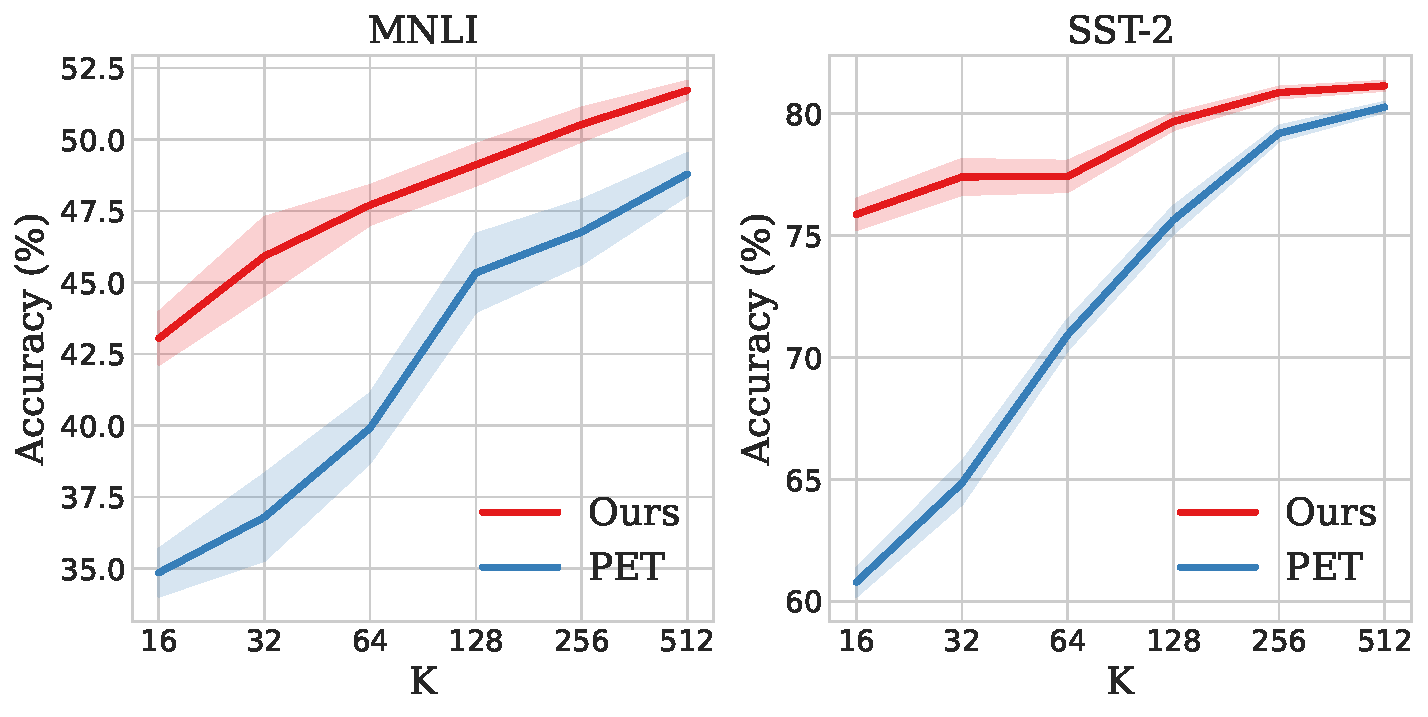
\includegraphics[width=\linewidth]{plot.pdf}
	\caption{Dataset scale analysis (\%).}
	\label{fig:dataset}
	\bigskip
\end{figure}

\noindent\textbf{Model Scale Analysis.}
%Similar to the previous experiment,
We test other sizes of BERT models and report the performance in Table~\ref{tab:model}. The statistics of these models are in~\cite{DBLP:journals/corr/abs-1908-08962}. We can also see the accuracy improvement is consistent when our distillation method is applied.
%Due to space limitation, we do not further elaborate here.
Hence, we suggest distilling from larger prompt-tuned models can benefit small models that can be efficiently deployed online.

\begin{table}
	\centering
	\begin{small}
		\begin{tabular}{l|ccc}
			\hline
			\bf Student Model & \bf SST-2 & \bf MPQA  & \bf MNLI  \\
			\hline
			BERT-base         & 66.1/87.8 & 67.2/84.0 & 40.4/51.5 \\
			BERT-small        & 62.5/77.5 & 63.9/74.3 & 34.8/43.3 \\
			BERT-tiny         & 56.8/62.4 & 60.6/67.1 & 33.6/34.8 \\
			\hline
		\end{tabular}
	\end{small}
	\caption{\label{tab:model} Model scale analysis (\%). $A/B$ refers to the model performance w/o and w/ KD, respectively.}
	\bigskip
\end{table}

\begin{table}[h!]
	\centering
	\begin{small}
		\begin{tabular}{l|l}
			\hline
			\bf Model            & \bf Top Tokens                            \\
			\hline
			Prompt-tuned Teacher & \textbf{great}, brilliant, good, $\cdots$ \\
			Pre-trained Teacher  & fun, \textbf{great}, good, $\cdots$       \\
			\hline
			{Prompt-Distiller}   & \textbf{great}, shaken, $\cdots$          \\
			\hline
		\end{tabular}
	\end{small}
	\caption{\label{tab:case} List of tokens generated by the MLM head with high probabilities where the input is ``it all adds up to good fun. it was [MASK].'' for sentiment analysis.}
\end{table}

\noindent\textbf{Case Study.}
In Table~\ref{tab:case}, we show a case for sentiment analysis where the results of both~{prompt-tuned} and~{pre-trained} teachers are listed, together with the student model.
It is evident both teachers provide sufficient knowledge for the student to learn, even for the zero-shot pre-trained teacher.

\section{Conclusion and Future Work}

In this work, we have presented~{Prompt-Distiller}, the first few-shot KD algorithm for prompt-based learners based on~{dual contrastive learning}.
It forces the student model to learn from both its~{pre-trained} and~{prompt-tuned} teacher models.
Experimental results over a variety of NLP tasks and datasets show that the~{Prompt-Distiller} framework consistently outperforms strong baselines by a large margin.
In the future, we would like to extend~{Prompt-Distiller} to other NLP tasks (such as text generation) and other large-scale PLMs (such as the GPT series).

\bigskip
\bigskip

\noindent\textbf{Acknowledgment.} This work is partially supported by the Alibaba Group through the Alibaba Innovative Research Program under Grant No. H20210412.

\newpage

\bibliographystyle{IEEEtran}
\bibliography{ref}

\end{document}